%!TEX root = ./main.tex

\section{Resugaring by Lazy Desugaring}
\label{sec3}

In this section, we present our new approach to resugaring. Different from the traditional approach that clearly separates the surface and the core languages, we combine them together as one mixed language, allowing users to freely use the language constructs in both languages. We will show that any expression in the mixed language can be evaluated in such a smart way that a sequence of all expressions that are necessarily to be resugared by the traditional approach can be correctly produced.

\subsection{Mixed Language for Resugaring}

\begin{figure}[thb]
	\[
	\begin{array}{lllll}
	 &\m{CoreExp} &::=& x  & \note{variable}\\
	       &&~|~& c  & \note{constant}\\
				 &&~|~& (\m{CoreHead'}~\m{CoreExp}_1~\ldots~\m{CoreExp}_n) & \note{constructor}\\
				 &&~|~& (\m{CommonHead}~\m{SurfExp}_1~\ldots~\m{SurfExp}_n) & \note{selected core constructor}\\
	\\
	 &\m{SurfExp} &::=& x  & \note{variable}\\
	       &&~|~& c  & \note{constant}\\
				 &&~|~& (\m{SurfHead}~\m{SurfExp}_1~\ldots~\m{SurfExp}_n) & \note{sugar expression}
	\end{array}
	\]
	\caption{Core and Surface Expressions}
	\label{fig:expression}
\end{figure}

We will define a mixed language for a given core language and a surface language defined over the core language. An expression in this language will be reduced step by step by the reduction rules for the core language and the desugaring rules for defining the syntactic sugars in the surface language.

\subsubsection{Core Language}

For our host language, we consider its evaluator as a blackbox %\todo{need to be corrected.} 
but with two natural assumptions. First, there is a deterministic stepper in the evaluator which, given an expression in the host language, can deterministically reduce the expression to a new expression. Second, the evaluation of any sub-expression has no side-effect on other parts of the whole expression.

An expression of the core language is defined in Figure \ref{fig:expression}. It is a variable, a constant, or a (language) constructor expression. Here, $\m{CoreHead}$ stands for a language constructor such as $\m{if}$ and $\m{let}$. To be concrete, we will use a simplified core language defined in Figure \ref{fig:core} to demonstrate our approach. \todo{semantic needed?}

\begin{figure}[thb]
\begin{centering}
	\framebox[36em][c]{
		\parbox[t]{33em}{
			\[
			\begin{array}{lcl}
			\m{CoreExp} &::=& \Code{(CoreExp~CoreExp)} ~~\note{// apply}\\
			&|& \m{(lambda~(x)~CoreExp)} ~~\note{// call-by-value}\\
			&|& \m{(lambdaN~(x)~CoreExp)} ~~\note{// call-by-need}\\
			&|& \m{(if~CoreExp~CoreExp~CoreExp)}\\
			&|& \m{(let~(x~CoreExp)~CoreExp)}\\
			&|& \m{(first~CoreExp)}\\
			&|& \m{(empty~CoreExp)}\\
			&|& \m{(rest~CoreExp)}\\
			&|& \m{(cons~CoreExp~CoreExp)}\\
			&|& \m{(arithop~CoreExp~CoreExp)} ~~\note{// +, -, *, /, >, <, =}\\
			&|& \m{x}\\
			&|& \m{c} ~~\note{// boolean, number and list}
			\end{array}
			\]
		}
	}
\end{centering}
\caption{An Core Language Example}
\label{fig:core}
\end{figure}


%For simplicity, we use the prefix notation. For instance, we write $\m{if-then-else}~e_1~e_2~e_3$, which would be more readable if we write $\m{if}~e_1~\m{then}~e_2~\m{else}~e_3$. In this paper, we may write both if it is clear from the context.

\subsubsection{Surface Language}

Our surface language is defined by a set of syntactic sugars, together with some basic elements in the core language, such as constant and variable. So an expression of the surface language is some core constructor expressions with sugar expressions, as defined in Figure \ref{fig:expression}.

A syntactic sugar is defined by a desugaring rule in the following form:
\[
\drule{(\m{SurfHead}~e_1~e_2~\ldots~e_n)}{\m{Exp}}
\]
where its LHS is a simple pattern (unnested) and its RHS is an expression of surface language or core language, and any subterms (e.g. $e_1$) in LHS only appear once in RHS. For instance, we may define syntactic sugar \m{And} by
\[
\drule{(\m{And}~e_1~e_2)}{(\m{if}~e_1~e_2~\false)}.
\]
Note that if the pattern is nested, we can introduce a new syntactic sugar to flatten it. And if we need a subterm multi times in RHS, a \m{let} binding is needed (a normal way in syntactic sugar).
One may wonder why \todo{don't understand..} not restricting the RHS to be a core expression $\m{CoreExp}$, which sounds more natural. We use $\m{surfExp}$ to be able to allow definition of recursive syntactic sugars, as seen in the following example.
\[
\begin{array}{l}
\drule{(\m{Odd}~e)}{(\m{if}~(>~e~0)~(\m{Even}~(-~e~1))~\false)}\\
\drule{(\m{Even}~e)}{(\m{if}~(>~e~0)~(\m{Odd}~(-~e~1))~\true)}
\end{array}
\]

We assume that all desugaring rules are not overlapped in the sense that for a syntactic sugar expression, only one desugaring rule is applicable.


\subsubsection{Mixed Language}

\begin{figure}[thb]
\begin{centering}
	\framebox[36em][c]{
		\parbox[t]{33em}{
			\[
			\begin{array}{lcl}
			\m{Exp} &::=& \m{DisplayableExp}\\
			&|& \m{UndisplayableExp}\\
\\
			\m{DisplayableExp} &::=& \m{SurfExp}\\
			&|& \m{CommonExp}
\\
			\m{UndisplayableExp} &::=& \m{CoreExp'}\\
			&|& \m{OtherSurfExp}\\
			&|& \m{OtherCommonExp}\\
\\
			\m{CoreExp} &::=& \m{CoreExp'}\\
						 &|& \m{CommonExp}\\
\\						
			\m{CoreExp'} &::=& (\m{CoreHead'}~\m{Exp}*)\\
\\
			\m{SurfExp} &::=& (\m{SurfHead}~\m{DisplayableExp}*)\\
\\
			\m{CommonExp} &::=& (\m{CommonHead}~\m{DisplayableExp}*)\\
			&|& c \qquad \note{// constant value}\\
			&|& x \qquad \note{// variable} \\
\\
			\m{OtherSurfExp} &::=& (\m{SurfHead}~\m{Exp}*~\m{UndisplayableExp}~\m{Exp}*)\\
\\
			\m{OtherCommonExp} &::=& (\m{CommonHead}~\m{Exp}*~\m{UndisplayableExp}~\m{Exp}*)
			\end{array}
			\]
		}
	}
\end{centering}
\caption{Our Mixed Language}
\label{fig:mix}
\end{figure}

Our mixed language for resugaring combines the surface language and the core language.
%
The differences between terms in our core language (CoreLang) and those in our surface language (SurfLang) are identified by their \m{Head}. But there may be some terms in the core language should be displayed during evaluation, or we need some core terms to help us getting better resugaring sequences . So we defined \m{CommonExp}, which origin from CoreLang, but can be displayed in resugaring sequences. The \m{Core'Exp} terms are terms with undisplayable \m{CoreHead} (named \m{CoreHead'}). The \m{SurfExp} terms are terms with \m{SurfHead} and all subexpressions are displayable. The \m{CommonExp} terms are terms with displayable CoreLang's \m{Head} (named \m{CommonHead}), together with displayable subexpressions. There exists some other expressions during our resugaring process, which have displayable \m{Head}, but one or more subexpressions should not display. They are \m{UndisplayableExp}. We distinct the two kinds of expression for \emph{abstraction} property (discussed in Section \ref{mark:abs}).

Take some terms in the core language in Figure \ref{fig:core} as examples.
We may assume \m{if}, \m{let}, \m{$\lambda _{N}$} (call-by-name lambda calculus), \m{empty}, \m{first}, \m{rest} as \m{CoreHead'}, \m{op}, \m{$\lambda$}, \m{cons} as \m{CommonHead}. Then we would show some useful intermediate steps.

Note that some expressions with \m{CoreHead} contains subexpressions with \m{SurfHead}, they are of \m{CoreExp} but not in core language, we need a tricky extension for the core language's evaluator.
We use $\redc{}{}$ to donate a reduction step of core language's expression, and $\rede{}{}$ to donate a step in the extension evaluator for the mixed language. We may use $\redm{}{}$ to donate one-step reduction in our mixed language, defined in the next section.
\infrule[CoreRed]
{ \forall~i.~e_i\in \m{CoreExp}\\
\redc{(\m{CoreHead}~e_1~\ldots~e_n)}{e'}}
{\rede{(\m{CoreHead}~e_1~\ldots~e_n)}{e'}}
\infrule[CoreExt1]
{ \forall~i.~subst_i= (e_i \in \m{SurfExp}~?~\m{tmpexp}~:~e_i),~where~\m{tmpexp}~is~any~reduciable~\m{CoreExp}\\
\redc{(\m{CoreHead}~subst_1~\ldots~subst_i~\ldots~subst_n)}{(\m{CoreHead}~subst_1~\ldots~subst_i'~\ldots~subst_n)}}
{\rede{(\m{CoreHead}~e_1~\ldots~e_i~\ldots~e_n)}{(\m{CoreHead}~e_1~\ldots~e_i'~\ldots~e_n)}\\where~\redm{e_i}{e_i'}~if~e_i~\in~\m{SurfExp},~else~\redc{e_i}{e_i'}}
\infrule[CoreExt2]
{ \forall~i.~subst_i= (e_i \in \m{SurfExp}~?~\m{tmpexp}~:~e_i),~where~\m{tmpexp}~is~any~reduciable~\m{CoreExp}\\
\redc{(\m{CoreHead}~subst_1~\ldots~subst_n)}{e'}~\note{// not reduced in subexpressions}}
{\rede{(\m{CoreHead}~e_1~\ldots~e_n)}{e'[e_1/subst_1~\ldots~e_n/subst_n]}}
For expression \Code{(CoreHead $e_1$ ... $e_n$)}, replacing all subexpression not in core language with any reducible core language's term \m{tmpexp}. Then getting a result after inputting the new expression \Code{e'} to the original blackbox stepper. If reduction appears at a subexpression at $e_i$ or what the $e_i$ replaced by, then the stepper with the extension should return \Code{(CoreHead $e_1$ ... $e_i'$ ... $e_n$)}, where $e_i'$ is $e_i$ after the mixed language's one-step reduction ($redm{}{}$) or after core language's reduction ($\redc{}{}$) (the rule \m{CoreExt1}, an example in Figure \ref{fig:e1}). Otherwise, stepper should return \Code{e'}, with all the replaced subexpressions replacing back. (the rule \m{CoreExt2}, an example in Figure \ref{fig:e2}) The extension will not violate properties of original core language's evaluator. It is obvious that the evaluator with the extension will reduce at the subexpression as it needs in core language, if the reduction appears in a subexpression. One may notice that the stepper with extension behaves the same as mixing the evaluation rules of core language and surface language. The extension is just to make it works when the evaluator of core language is a blackbox stepper. That's why the extension is tricky.

\begin{center}
\begin{figure}[thb]
\centering
\Code{(if (and e1 e2) true false)}\\ $\Downarrow_{replace}$\\ \Code{(if tmpe1 true false)}\\ $\Downarrow_{blackbox}$\\ \Code{(if tmpe1' true false)}\\ $\Downarrow_{desugar}$\\ \Code{(if (if e1 e2 false) true false)}
\caption{\m{CoreExt1}'s example}
\label{fig:e1}
\end{figure}

\begin{figure}[thb]
\centering
\Code{(if (if true ture false) (and ...) (or ...))}\\ $\Downarrow_{replace}$ \\\Code{ (if (if true ture false) tmpe2 tmpe3)}\\ $\Downarrow_{blackbox}$\\  \Code{(if true tmpe2 tmpe3)}\\ $\Downarrow_{replaceback}$\\ \Code{(if true (and ...) (or ...))}
\caption{\m{CoreExt2}'s example}
\label{fig:e2}
\end{figure}


 % \Code{(if true (and ...) (or ...))} $\Rightarrow_{replace}$ \Code{(if true tmpe2 tmpe3)} $\Rightarrow_{blackbox}$ \\ \Code{tmpe2} $\Rightarrow_{replaceback}$ \Code{(and ...)}

\end{center}

\subsection{Resugaring Algorithm}

Our resugaring algorithm works on our mixed language, based on the reduction rules of the core language and the desugaring rules for defining the surface language. Let $\rede{}{}$ denote the one-step reduction of the core language (based on the blackbox stepper with extension), and $\drule{}{}$ the one-step desugaring of outermost sugar. We define $\redm{}{}$, the one-step reduction of our mixed language, as follows.

\label{mark:miexedreduction}
\infrule[ExtRed]
{\rede{(\m{CoreHead}~e_1~\ldots~e_n)}{e'}}
{\redm{(\m{CoreHead}~e_1~\ldots~e_n)}{e'}}

\infrule[SurfRed1]
{\drule{(\m{SurfHead}~x_1~\ldots~x_i~\ldots~x_n)}{e},~\redm{e_i}{e_i''}\\
\exists i.\, \redm{e[e_1/x,\ldots,e_i/x_i,\ldots,e_n/x_n]}{e[e_1/x,\ldots,e_i'/x_i,\ldots,e_n/x_n]}
}
{\redm{(\m{SurfHead}~e_1~\ldots~e_i~\ldots~e_n)}{(\m{SurfHead}~e_1~\ldots~e_i''~\ldots~e_n)}}

\infrule[SurfRed2]
{\drule{(\m{SurfHead}~x_1~\ldots~x_i~\ldots~x_n)}{e}\\
\neg \exists i.\, \redm{e[e_1/x_1,\ldots,e_i/x_i,\ldots,e_n/x_n]}{e[e_1/x_1,\ldots,e_i'/x_i,\ldots,e_n/x_n]}
}
{\redm{(\m{SurfHead}~e_1~\ldots~e_i~\ldots~e_n)}{e[e_1/x_1,\ldots,e_i/x_i,\ldots,e_n/x_n]}
}

The \m{CoreRed} rule describes how our mixed language handles expressions with \m{CoreHead}---just leave it to the core language's evaluator with the extension. Then for the expression with \m{SurfHead}, we will firstly desugar the outermost sugar (identified by the \m{SurfHead}), then recursively executing $\redm{}{}$. In the recursive call, if one of original subexpression $e_i$ is reduced (\m{SurfRed1}), then the original sugar is not necessarily desugared, we should only reduce the subexpression $e_i$; if not (\m{SurfRed2}), then the sugar have to desugar.

%\todo{Add explanantion of the above rule.}

Then our desugaring algorithm is defined based on $\redm{}{}$.

\[
\begin{array}{llll}
\m{resugar} (e) &=& \key{if}~\m{isNormal}(e)~\key{then}~return\\
              & & \key{else}~\\
							& & \qquad \key{let}~\redm{e}{e'}~\key{in}\\
							& & \qquad \key{if}~e' \in~\m{DisplayableExp} \\
							& & \qquad \qquad \m{output}(e'),~\m{resugar}(e')\\
							& & \qquad \key{else}~\m{resugar}(e')
\end{array}
\]

During the resugaring, we just call the mixed language's reduction ($\redm{}{}$) on the input expression until the expression becomes a normal form. We use the \m{DisplayableExp} to restrict immediate sequences to be output or not. It is more explicit compared to existing approaches. And because $\redm{}{}$ will be executed recursively on the subexpressions, it can be optimized. (see in \ref{mark:optimize}, because the current description is more easier to understand.)

\subsection{Correctness}
\label{mark:correct}

Existing resugaring works\cite{resugaring,hygienic} define three properties for correctness of resugaring. We think they are also reasonable to describe correctness of our approach. We describe the following properties in our mixed language's domain, then prove or discuss on them.

\emph{Emulation.} For each reduction of an expression in our mixed language, it should reflect on one step reduction of the expression totally desugared in the core language, or one step desugaring on a syntactic sugar.

\emph{Abstraction.} Only displayable expressions defined in our mixed language appear in our resugaring sequences.

\emph{Coverage.} No syntactic sugar is desugared before its sugar structure should be destroyed in core language.

\subsubsection{Emulation} It is a basic property for correctness. Since desugaring won't change an expression after totally desugared, what we need to prove is that a non-desugaring reduction in the mixed language shows the exactly reduction which should appear after the expression totally desugared. We express it by following lemma. (\m{fulldesugar}(\m{exp}) returns the expression after \m{exp} totally desugared)

\begin{lemma}
\label{lemma1}

For~\m{exp}=$(\m{SurfHead}~e_1~\ldots~e_i~\ldots~e_n)\in\m{SurfExp}$, if~$\redm{\m{exp}}{\m{exp'}}$\\ and \m{fulldesugar}(\m{exp})$\not=$$\m{fulldesugar}(\m{exp'})$,~then $\redc{\m{fulldesugar}(\m{exp})}{\m{fulldesugar}(\m{exp'})}$

\end{lemma}

\begin{Def}[Emulation]
If the mixed language satisfies Lemma \ref{lemma1}, then the resugaring satisfies emulation property.
\end{Def}

\begin{lemma}
\label{lemma2}

For~\m{exp} = $(\m{SurfHead}~e_1~\ldots~e_i~\ldots~e_n)$, if inputting $\m{fulldesugar}(\m{exp})$ to core language's evaluator reduces the term original from $e_i$ in one step, then the $\redm{}{}$ will reduce \m{exp} at $e_i$.

%then $\redc{\m{fulldesugar}(\m{Exp})}{\m{fulldesugar}(\m{Exp'})}$
\end{lemma}

\begin{proof}[Proof of Lemma \ref{lemma2}]
For $\drule{(\m{SurfHead}~x_1~\ldots~x_i~\ldots~x_n)}{e}$

if $e$ is of normal form, the $\m{fulldesugar}(\m{exp})$ will not be reduced by core evaluator.

if $e$ is headed with \m{CoreHead}, then according to the \m{CoreRed} rule, the $\rede{}{}$ will execute on $e$ according to \m{ExtRed}, which will reduce the subexpression $e_i$ according to the blackbox evaluator with extension. Then the \m{SurfRed2} rule will reduce $e_i$. Because of the extension of evaluator reduces the subexpression in correct location, so it is for $\redm{}{}$.

if $e$ is headed with \m{SurfHead}, then the $redm{}{}$ will execute recursively on $e$. If the new one satisfies the lemma, then it is for the former. Because any sugar expression will finally be able to desugar to expression with \m{CoreHead}, it can be proved recursively.
\end{proof}
\begin{proof}[Proof of Lemma \ref{lemma1}]
\hfill

For \m{SurfRed1} rule, $\redm{(\m{SurfHead}~e_1~\ldots~e_i~\ldots~e_n)}{(\m{SurfHead}~e_1~\ldots~e_i''~\ldots~e_n)}$, where $\redm{e_i}{e_i''}$. 
If $\m{fulldesugar}(e_i)$=$\m{fulldesugar}(e_i'')$, then \m{fulldesugar}(\m{Exp})=\m{fulldesugar}(\m{Exp'}). If not,  what we need to prove is that, $\redc{\m{fulldesugar}(\m{Exp})}{\m{fulldesugar}(\m{Exp'})}$. Note that the only difference between \m{Exp} and \m{Exp'} is the i-th subexpression, and we have proved the lemma \ref{lemma2} that the subexpression is the one to be reduced after the expression desugared totally, it will be also a recursive proof on the subexpression $e_i$.

For \m{SurfRed2} rule, \m{Exp'} is \m{Exp} after the outermost sugar resugared. So \m{fulldesugar}(\m{Exp})=

\begin{flushleft}
\m{fulldesugar}(\m{Exp'}).
\end{flushleft}

\end{proof}

So our resugaring approach satisfies evaluation property.

\subsubsection{Abstraction}
\label{mark:abs}

Abstraction is not a restrict properties, because each expression has its meaning. Users may choose what they want to output during the process. Existing resugaring approaches use marks to determine whether to display a term generated by desugaring, or only changes on original terms will show.

We define the abstraction by catalog the expression in the mixed language, from the reason why we need resugaring---sugar expressions become unrecognizable after desugaring. So why cannot a recursive sugar's resugaring sequences show the sugars generated by itself? We think the users should be allowed to decide which terms are recognizable. Then during the resugaring process, if no unrecognizable term for the user appears in the whole expression, the expression should be shown as a step in resugaring sequences. Lazy resugaring, as the key idea of our approach, makes any intermediate steps retain as many sugar structures as possible, so the abstraction is easy.

\subsubsection{Coverage}
The coverage property is important, because resugaring sequences are useless if lose intermediate steps. By lazy desugaring, it becomes obvious, because there is no chance to lose. In Lemma \ref{lemma3}, we want to show that our reduction rules in the mixed language is \emph{lazy} enough. Because it is obvious, we only give a proof sketch here.
\begin{lemma}
\label{lemma3}
A syntactic sugar only desugars when \emph{necessary}, that means after a reduction on the fully-desugared expression, the sugar's structure is destroyed.
\end{lemma}

\begin{Def}[Coverage]
If the reduction of mixed language satisfies Lemma \ref{lemma3}, then the resugaring satisfies coverage property.
\end{Def}



\begin{proof}[Proof sketch of Lemma \ref{lemma3}]
From Lemma \ref{lemma2}, we know the $\redm{}{}$ recursively reduces a expression at correct subexpression. Or the $\redm{}{}$ will destroy the outermost sugar (of the current expression) in rule \m{SurfRed2}. Note that it is the only rule to desugar sugars directly (other rules only desugar sugars when recursively call \m{SurfRed2}), we can prove the lemma recursively if \m{SurfRed1} is \emph{lazy} enough.

In \m{SurfRed2} rule, we firstly expand the outermost sugar and get a temp expression with structure of the outermost sugar. Then when we recursively call $\redm{}{}$, the reduction result shows the structure has been destroyed, so the outermost sugar has to be desugared. Since the recursive reduction of a terminable (Some bad sugars may never stop which are pointless.) sugar expression will finally terminate, the lemma can be proved recursively.
\end{proof}



\subsection{Implementation}

Our resugaring approach is implemented using PLT Redex\cite{SEwPR}, which is an semantic engineering tool based on reduction semantics\cite{reduction}. The framework of the implementation is as Figure \ref{fig:frame}.

\begin{figure}[thb]
	\centering
	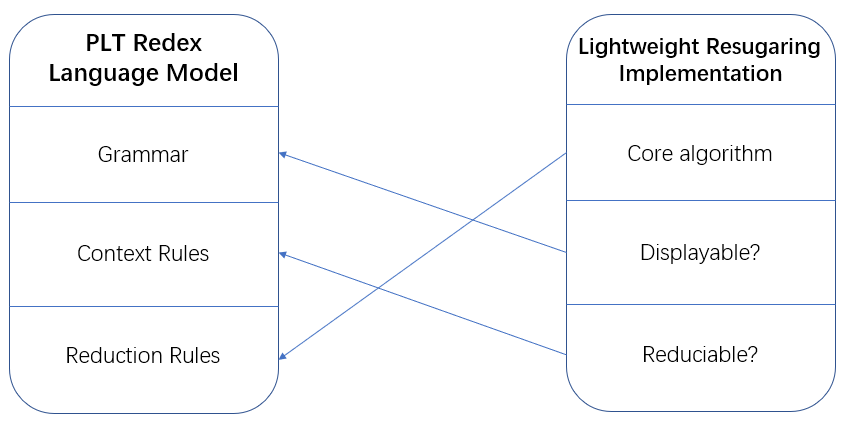
\includegraphics[width=8cm]{images/frame.png}
	\caption{framework of implementation}
	\label{fig:frame}
\end{figure}

Instead of implementing a blackbox stepper of core language, we just used the core language's reduction semantics, because its behavior is same as the stepper with extension for mixed language. We have proved or discussed the correctness with the assumption that the core language's evaluator is a blackbox stepper. In the language model, desugaring rules are written as reduction rules of \m{SurfExp}. And context rules of \m{SurfExp} have no restrict (every subexpressions is reducible as a hole). Then for each resugaring step, we should choose the exact reduction which satisfies the reduction of mixed language's rule (see in section \ref{mark:miexedreduction}).

\label{mark:optimize}
Note that in \m{SurfRed1} rule and \m{CoreExt1} rule, there is a recursive call on $\redm{}{}$. We can optimize the resugaring algorithm by recursively resugaring. For example, \Code{(Sugar1 (Sugar2 e21 e22 ...) e11 e12 ...)} as the input, and find the first subexpression should be reduced. We can firstly get the resugaring sequences of \Code{(Sugar2 e21 e22)}
\begin{Codes}
    (Sugar2 e21 e22 ...)
\OneStep{ exp1}
\DeStep{  exp...} \note{// may be 0 or more steps}
\OneStep{ expn}
\end{Codes}
Then a resugaring subsequence is got as
\begin{Codes}
    (Sugar1 (Sugar2 e21 e22 ...) e11 e12 ...)
\OneStep{ (Sugar1 exp1 e11 e12 ...)}
\DeStep{  (Sugar1 exp... e11 e12 ...)} \note{// may be 0 or more steps}
\OneStep{ (Sugar1 expn e11 e12 ...)}
\end{Codes}
Thus, we will not need to try to expand the outermost sugar for each inner step (recursively resugaring for inner expression).

% The grammar of the whole language contains Coreexp', Surfexp and Commonexp as the language setting in sec\ref{sec3}. OtherSurfexp is of Surfexp and OtherCommonexp is of Commonexp. The identifier of any kind of expression is Headid of expression. If we need to add a syntactic sugar to the whole language, only three steps is needed.

% \begin{enumerate}
% \item Add grammar of the syntactic sugar.
% \item Add context rules of the sugar, such that any sub-expressions can be reduced.
% \item Add desugar rules of the sugar to reduction rules of the whole language.
% \end{enumerate}

% Then inputting an expression of the syntactic sugar to lightweight-resugaring will get the resugaring sequences.

\subsection{Application}

We test some applications on the tool. Note that we set call-by-value lambda calculus as terms in \m{CommonExp}, because we need to output some intermediate sequences including lambda expressions in some examples. It's easy if we want to skip them.

\subsubsection{simple sugar}
\label{mark:simple}

We construct some simple syntactic sugars and try it on our tool. Some sugar is inspired by the first work of resugaring\cite{resugaring}. The result shows that our approach can handle all sugar features of their first work.

We take a SKI combinator syntactic sugar as an example. We will show why our approach is lightweight.
\[
\begin{array}{l}
\drule{\m{S}}{\Code{(lambdaN (x1 x2 x3) (x1 x2 (x1 x3)))}}\\
\drule{\m{K}}{\Code{(lambdaN (x1 x2) x1)}}\\
\drule{\m{I}}{\Code{(lambdaN (x) x)}}
\end{array}
\]

% \begin{Codes}
% 	S \DeStep{ (lambdaN (x1 x2 x3) (x1 x2 (x1 x3)))}
% 	K \DeStep{ (lambdaN (x1 x2) x1)}
% 	I \DeStep{ (lambdaN (x) x)}
% \end{Codes}



Although SKI combinator calculus is a reduced version of lambda calculus, we can construct combinators' sugar based on call-by-need lambda calculus in our CoreLang. For sugar expression \Code{(S (K (S I)) K xx yy)}, we get the following resugaring sequences.
\begin{Codes}
    (S (K (S I)) K xx yy)
\OneStep (((K (S I)) xx (K xx)) yy)
\OneStep (((S I) (K xx)) yy)
\OneStep (I yy ((K xx) yy))
\OneStep (yy ((K xx) yy))
\OneStep (yy xx)
\end{Codes}


For the existing approach, the sugar expression should firstly desugar to
\begin{Codes}
((lambdaN
   (x1 x2 x3)
   (x1 x3 (x2 x3)))
  ((lambdaN (x1 x2) x1)
   ((lambdaN
     (x1 x2 x3)
     (x1 x3 (x2 x3)))
    (lambdaN (x) x)))
  (lambdaN (x1 x2) x1)
  xx yy)
\end{Codes}

Then in our CoreLang, the execution of expanded expression will contain 33 steps. For each step, there will be many attempts to match and substitute the syntactic sugars to resugar the expression. It will omit more steps for a larger expression.
So the unidirectional resugaring algorithm makes our approach lightweight, because no attempts for resugaring the expression are needed.
\subsubsection{hygienic sugar}
\label{mark:hygienic}


The second work\cite{hygienic} of existing resugaring approach mainly processes hygienic sugar compared to first work. It use a DAG to represent the expression. However, hygiene is not hard to handle by our lazy desugaring strategy. Our algorithm can easily process hygienic sugar without special data structure. 


A typical hygienic problem is as the following example.
\[
\drule{\Code{(Hygienicadd e1 e2)}}{\Code{(let (x e1) (+ x e2))}}
\]
% \begin{Codes}
% 	(Hygienicadd e1 e2) \DeStep{ (let ((x e1)) (+ x e2))}
% \end{Codes}

For existing resugaring approach, if we want to get sequences of \Code{(let ((x 2)) (Hygienicadd 1 x))}, it will firstly desugar to \Code{(let ((x 2)) (let ((x 1)) (+ x x)))}, which is awful because the two $x$ in \Code{(+ x x)} should be bind to different value. So existing hygienic resugaring approach use abstract syntax DAG to distinct different \m{x} in the desugared expression. But for our approach based on lazy desugaring, the \m{hygienicadd} sugar does not have to desugar until necessary, so, getting following sequences based on a hygienic rewriting system.

\begin{Codes}
    (let ((x 2)) (Hygienicadd 1 x)
\OneStep{ (Hygienicadd 1 2)}
\OneStep{ (+ 1 2)}
\OneStep{ 3}
\end{Codes}

The lazy desugaring is also convenient for hygienic resugaring for non-hygienic rewriting. For example, \Code{(let ((x 1)) (+ x (let ((x 2)) (+ x 1))))} may be reduced to \Code{(+ 1 (let ((1 2)) (+ 1 1)))} by a simple core language whose \Code{let} expression does not handle cases like that. But by writing a simple sugar Let,
\[\drule{\Code{(Let~e1~e2~e3)}}{\Code{(let~((e1~e2))~e3)}}\]
and some simple modifies in the reduction of mixed language, we will get the following sequences in our system.
\begin{Codes}
    (Let x 1 (+ x (Let x 2 (+ x 1))))
\OneStep{ (Let x 1 (+ x (+ 2 1)))}
\OneStep{ (Let x 1 (+ x 3))}
\OneStep{ (+ 1 3)}
\OneStep{ 4}
\end{Codes}

In practical application, we think hygiene can be easily processed by rewriting system, so we just use a rewriting system which can rename variable automatically. But our result shows lazy desugaring is really a good way to handle hygienic sugar in any systems.

\subsubsection{recursive sugar}
Recursive sugar is a kind of syntactic sugars where call itself or each other during the expanding. For example,
\[
\begin{array}{l}
\drule{(\m{Odd}~e)~}{\Code{(if (> e 0) (Even (- e 1)) \false)}}\\
\drule{(\m{Even}~e)}{\Code{(if (> e 0) (Odd (- e 1)) \true)}}
\end{array}
\]
are common recursive sugars. The existing resugaring approach can't process syntactic sugar written as this (non pattern-based) easily, because boundary conditions are in the sugar itself.

Take $(Odd~2)$ as an example. The previous work will firstly desugar the expression using the rewriting system. Then the rewriting system will never terminate as following shows.
\begin{Codes}
   (Odd 2)
\DeStep{ (if (> 2 0) (Even (- 2 1) \#f))}
\DeStep{ (if (> (- 2 1) 0) (Odd (- (- 2 1) 1) \#t))}
\DeStep{ (if (> (- (- 2 1) 1) 0) (Even (- (- (- 2 1) 1) 1) \#f))}
\DeStep{ ...}
\end{Codes}


Then the advantage of our approach is embodied. Our lightweight approach doesn't require a whole expanding of sugar expression, which gives the framework chances to judge boundary conditions in sugars themselves, and showing more intermediate sequences. We get the resugaring sequences of the former example using our tool.
\begin{Codes}
    (Odd 2)
\OneStep{ (Even (- 2 1))}
\OneStep{ (Even 1)}
\OneStep{ (Odd (- 1 1))}
\OneStep{ (Odd 0)}
\OneStep{ \#f}
\end{Codes}


We also construct some higher-order syntactic sugars and test them. The higher-order feature is important for constructing practical syntactic sugars. And many higher-order sugars should be constructed by recursive definition. The first sugar is \m{filter}, implemented by pattern matching term rewriting.
\[\Code{(filter e (list v1 v2 ...))}\]
\[
\drule{}
{\Code{(if (e v1) (cons v1 (filter e (list v2 ...)))\ (filter e (list v2 ...)))}}
\]
\[
\drule{\Code{(filter e (list))}}{\Code{(list)}}
\]
and getting the following result. (by making \Code{(lambda ...)} \m{CommonExp} )

\begin{Codes}
    (filter (lambda (x) (and (> x 1) (< x 4))) (list 1 2 3 4))
\OneStep{ (filter (lambda (x) (and (> x 1) (< x 4))) (list 2 3 4))}
\OneStep{ (cons 2 (filter (lambda (x) (and (> x 1) (< x 4))) (list 3 4)))}
\OneStep{ (cons 2 (cons 3 (filter (lambda (x) (and (> x 1) (< x 4))) (list 4))))}
\OneStep{ (cons 2 (cons 3 (filter (lambda (x) (and (> x 1) (< x 4))) (list))))}
\OneStep{ (cons 2 (cons 3 (list)))}
\OneStep{ (cons 2 (list 3))}
\OneStep{ (list 2 3)}
\end{Codes}

Here, although the sugar can be processed by existing resugaring approach, it will be redundant. The reason is that, a filter for a list of length $n$ will match to find possible resugaring $n*(n-1)/2$ times. Thus, lazy desugaring is really important to reduce the resugaring complexity of recursive sugar.

Moreover, just like the \emph{Odd and Even} sugar above, there are some simple rewriting systems which do not allow pattern-based rewriting. Or there are some sugars which need to be expressed by the terms in core language as rewriting conditions. Take the example of another higher-order sugar \m{map} as an example.
\[
\begin{array}{l}
\drule{\Code{(map e1 e2)}}{}\\
\Code{(let ((x e2)) (if (empty x) (list) (cons (e1 (first x)) (map e1 (rest x)))))}
\end{array}
\]

Get following resugaring sequences.
\begin{Codes}
    (map (lambda (x) (+ x 1)) (cons 1 (list 2)))
\OneStep{ (map (lambda (x) (+ x 1)) (list 1 2))}
\OneStep{ (cons 2 (map (lambda (x) (+ 1 x)) (list 2)))}
\OneStep{ (cons 2 (cons 3 (map (lambda (x) (+ 1 x)) (list))))}
\OneStep{ (cons 2 (cons 3 (list)))}
\OneStep{ (cons 2 (list 3))}
\OneStep{ (list 2 3)}
\end{Codes}

Note that the \m{let} term is to limit the subexpression only appears once in RHS. In this example, we can find that the list \Code{(cons 1 (list 2))}, though equal to \Code{(list 1 2)}, is represented by core language's term. So it will be difficult to handle such inline boundary conditions by rewriting system. But our approach is easy to handle cases like this.

\subsection{Compare to previous work}

As mentioned many times before, the biggest difference between previous resugaring approach and our approach, is that our approach doesn't need to desugar the sugar expression totally. Thus, our approach has the following advantages compared to previous work.

\begin{itemize}
	\item \emph{Lightweight and efficient.} Our approach does not need tags to mark desugaring information as existing approaches, and only unidirectional desugaring is needed, so it is a lightweight approach. As the example at sec\ref{mark:simple}, the match and substitution process searches all intermediate sequences many times. It will cause huge cost for a large program. So out approach---only expanding a syntactic sugar when necessarily, is a efficient approach.
	\item \emph{Friendly to hygienic sugar} Previous hygienic resugaring approach use a new data structure to process resugaring of hygienic sugar. Our approach simply desugar the sugars 
	\item \emph{More syntactic sugar features} The ability of processing non-pattern-based (\todo{inline?}) recursive sugar is a superiority compared to previous work. The key point is that recursive syntactic sugar must handle boundary conditions. Our approach handle them easily by not necessarily desugaring all syntactic sugars. Higher-order functions, as an important feature of functional programming, was supported by many daily programming languages. Lazy desugaring makes writing higher-order sugars easier.
	\item \todo{easier sugar?}
	% \item {\emph Rewriting rules based on reduction semantics} Any syntactic sugar that can expressed by reduction semantics can be used in our approach. It will give more possible forms for constructing syntactic sugars. todo:example?
\end{itemize}

